\section{Trazado de Conos con Vóxeles} % (fold)
\label{sec:trazado_de_conos}
El trazado de conos es utilizado para distintos aspectos visuales de la aplicación. En nuestra implementación este proceso se realiza durante el cálculo de iluminación utilizando sombreado diferido (sección \ref{sub:deferred_rendering_theory}). Utilizar sombreado diferido es muy conveniente ya que durante el cálculo de iluminación solo es necesario trazar conos sobre cada píxel en vez de cada fragmento incluyendo los no visibles.

Como se menciona en la sección \ref{sec:trazado_de_conos_con_voxeles}. El trazado de conos es similar a ray-marching con la única diferencia que el volumen a muestrear incrementa de tamaño según la distancia recorrida. Esto es producto de la expansión de la apertura del cono a través de su expansión. Las muestras de mayor tamaño se obtienen utilizando los niveles de mipmap descritos en la sección anterior.

Al utilizar vóxeles anisótropos se necesita saber que volúmenes direccionales van a ser utilizados para muestrear a través del recorrido del cono. Esto se determina según el signo de cada eje del vector direccional del cono. También es necesario calcular el peso de cada eje para obtener un resultado ponderado entre los tres volúmenes. El Código \ref{Trace0} describe este proceso.
\\
\begin{lstlisting}[caption={Lógica para determinar volúmenes direccionales a utilizar durante el trazado de conos y peso por eje.}, label=Trace0]
vec4 TraceCone(vec3 position, vec3 normal, vec3 direction, float aperture)
{
    // índice de los tres volúmenes direccionales
    uvec3 visibleFace;
    // selección de índices según el signo
    visibleFace.x = (direction.x < 0.0) ? 0 : 1;
    visibleFace.y = (direction.y < 0.0) ? 2 : 3;
    visibleFace.z = (direction.z < 0.0) ? 4 : 5;
    // peso por eje de la dirección del cono
    vec3 weight = direction * direction;
(*@\centerline{\raisebox{-1pt}[0pt][0pt]{$\vdots$}}@*)
}
\end{lstlisting}

Durante el recorrido del cono se utiliza la función de GLSL \emph{textureLod}. Esta función tiene como entrada una textura, una coordenada y un nivel mip. Durante la marcha del cono el nivel mip se obtiene del diámetro del cono dado una distancia desde el origen:
\begin{equation}
    V_{level} = \log_2\left(\frac{d}{V_{size}}\right)
\end{equation} donde $d$ es el diámetro del círculo del cono según la distancia recorrida y $V_{size}$ es el tamaño de un vóxel en la cuadrícula de vóxeles en el máximo nivel de detalle. El valor de $d$ se puede obtener de la siguiente ecuación:
\begin{equation}
    d = 2t\cdot\tan\left(\frac{\theta}{2}\right)
\end{equation} donde $t$ es la distancia recorrida por el cono desde el punto de origen y $\theta$ es el ángulo de apertura del cono. En la Figura \ref{fig:cone_trace_impl_fi} se observa una representación visual de este recorrido:
\begin{figure}[H]
    \centering
    \captionsetup{justification=centering}
    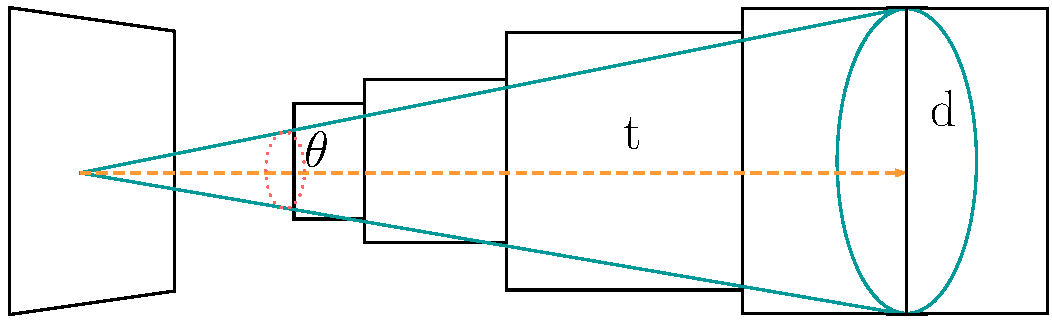
\includegraphics[width=.9\linewidth]{media/cone.pdf}
    \caption{Visualización del recorrido de un cono.}
    \label{fig:cone_trace_impl_fi}
\end{figure}

En nuestra implementación el punto de origen del cono es trasladado según el tamaño de un vóxel. El Código \ref{Trace1} expone esta operación. Esto se hace para evitar que el cono colisione con el vóxel de origen.
\\
\begin{lstlisting}[caption={Traslado de origen del cono.}, label=Trace1]
vec4 TraceCone(vec3 position, vec3 normal, vec3 direction, float aperture)
{
(*@\centerline{\raisebox{-1pt}[0pt][0pt]{$\vdots$}}@*)
    // distancia inicial recorrida de un vóxel 
    float dst = voxelWorldSize;
    // posición inicial
    vec3 startPosition = position + normal * dst;
(*@\centerline{\raisebox{-1pt}[0pt][0pt]{$\vdots$}}@*)
}
\end{lstlisting}

Finalmente se comienza el trazado del cono a través de la escena. Este es expuesto en el Código \ref{Trace2}.
\\
\begin{lstlisting}[caption={Trazado de cono con vóxeles.}, label=Trace2]
// volumen de radiancia o textura base
layout(binding = 7) uniform sampler3D voxelTex;
// volúmenes direccionales
layout(binding = 8) uniform sampler3D voxelTexMipmap[6];
// obtiene una muestra de la representación en vóxeles
vec4 AnistropicSample(vec3 coord, vec3 weight, uvec3 face, float lod)
{
    // nivel mip en los volúmenes direccionales
    float anisoLevel = max(lod - 1.0f, 0.0f);
    // muestra direccional ponderada por el peso de cada eje
    vec4 anisoSample = weight.x * textureLod(voxelTexMipmap[face.x], coord, anisoLevel)
                     + weight.y * textureLod(voxelTexMipmap[face.y], coord, anisoLevel)
                     + weight.z * textureLod(voxelTexMipmap[face.z], coord, anisoLevel);

    // interpolación lineal con la textura base 
    // cuando el nivel de detalle es menor a 1
    if(lod < 1.0f)
    {
        vec4 baseColor = texture(voxelTex, coord);
        anisoSample = mix(baseColor, anisoSample, clamp(lod, 0.0f, 1.0f));
    }

    return anisoSample;                    
}
vec4 TraceCone(vec3 position, vec3 normal, vec3 direction, float aperture)
{
(*@\centerline{\raisebox{-1pt}[0pt][0pt]{$\vdots$}}@*)
    // resultado de acumulación
    vec4 coneSample = vec4(0.0f);
    // máxima distancia para el recorrido de un cono
    float maxDistance = maxTracingDistanceGlobal / voxelScale

    while(coneSample.a < 1.0f && dst <= maxDistance)
    {
        vec3 conePosition = startPosition + direction * dst;
        // expansión del diámetro del cono
        float diameter = 2.0f * aperture * dst;
        // nivel de detalle según el diámetro
        float mipLevel = log2(diameter / voxelWorldSize);
        // conversión de posición en espacio de mundo a espacio de textura
        vec3 coord = WorldToVoxel(conePosition);
        // muestra anisotrópica
        vec4 anisoSample = AnistropicSample(coord, weight, visibleFace, mipLevel);
        // composición front-to-back
        coneSample += (1.0f - coneSample.a) * anisoSample;
        // aumento de la distancia recorrida
        dst += diameter * samplingFactor;
    }

    return coneSample;
}
\end{lstlisting}

En el método \emph{AnistropicSample} se puede observar el muestreo direccional, ponderado por el peso de cada eje en la dirección del cono y el uso de la función \emph{mix()} para interpolar entre los volúmenes direccionales y la textura base. 

Durante el trazado se observa cómo se obtiene la posición del cono según la distancia recorrida y el uso de las operaciones ya mencionadas para obtener el diámetro y el nivel mip. La función \emph{WorldToVoxel} aparece para cambiar una posición en espacio de mundo a espacio de textura como fue mencionado para el Código \ref{SpaceTransform}. La distancia recorrida es alterada por una variable \emph{samplingFactor} esto permite disminuir la distancia entre muestreos para lograr resultados más suaves con un costo en rendimiento.

Para acumular los valores muestreados través del recorrido del cono se utiliza acumulación volumétrica \emph{front-to-back}. Para esto es necesario llevar pista de un valor oclusión $a$ y color $c$. La actualización de estos valores por cada paso con un nuevo valor $a_2$ y $c_2$ se realiza de la siguiente manera: $c=c+(1-a)c_2$ y $a=a+(1-a)a_2$. En el algoritmo se puede observar que esto se realiza con la variable \emph{coneSample}.

\subsection{Reflexión Difusa} % (fold)
\label{sub:reflexion_difuse}
Para el cálculo de reflexión difusa se utilizan seis conos dentro de la semiesfera orientada por el vector normal como se describen en la Figura \ref{fig:brdf_cones2}. El Código \ref{Trace3} demuestra el proceso de integracion de los conos difusos.
\\
\begin{lstlisting}[caption={Conos para reflexión difusa.}, label=Trace3]
// direcciones de conos difusos
const vec3 diffuseConeDirections[] =
{
    vec3(0.0f, 1.0f, 0.0f),
    vec3(0.0f, 0.5f, 0.866025f),
    vec3(0.823639f, 0.5f, 0.267617f),
    vec3(0.509037f, 0.5f, -0.7006629f),
    vec3(-0.50937f, 0.5f, -0.7006629f),
    vec3(-0.823639f, 0.5f, 0.267617f)
};
// pesos de conos difusos
const float diffuseConeWeights[] =
{
    PI / 4.0f,
    3.0f * PI / 20.0f,
    3.0f * PI / 20.0f,
    3.0f * PI / 20.0f,
    3.0f * PI / 20.0f,
    3.0f * PI / 20.0f,
};
vec4 CalculateIndirectLighting(vec3 position, vec3 normal, vec3 albedo, vec4 specular)
{
    // resultado de integración del trazado difuso
    vec4 diffuseTrace = vec4(0.0f);
    // dirección del cono
    vec3 coneDirection = vec3(0.0f);
(*@\centerline{\raisebox{-1pt}[0pt][0pt]{$\vdots$}}@*)
    // albedo es mayor a cero, si albedo es cero no hay radiancia
    if(any(greaterThan(albedo, diffuseTrace.rgb)))
    {
        // apertura del cono es la tangente del ángulo medio
        const float aperture = 0.57735f // tan(60/2);
        // vector guía para obtener vectores direccionales arbitrarios
        vec3 guide = vec3(0.0f, 1.0f, 0.0f);

        if (abs(dot(normal,guide)) == 1.0f)
        {
            guide = vec3(0.0f, 0.0f, 1.0f);
        }

        // obtener hacia la derecha y hacia arriba
        vec3 right = normalize(guide - dot(normal, guide) * normal);
        vec3 up = cross(right, normal);

        for(int i = 0; i < 6; i++)
        {
            // rotación de la dirección según cada dirección del cono difuso con vector normal
            coneDirection = normal;
            coneDirection += diffuseConeDirections[i].x * right + diffuseConeDirections[i].z * up;
            coneDirection = normalize(coneDirection);
            // se acumula el resultado de cada cono y se hace un ponderado por peso
            diffuseTrace += TraceCone(position, normal, coneDirection, aperture) * diffuseConeWeights[i];
        }

        diffuseTrace.rgb *= albedo;
    }
(*@\centerline{\raisebox{-1pt}[0pt][0pt]{$\vdots$}}@*)
}
\end{lstlisting}

Las direcciones, pesos de integración y tangente del ángulo ya se encuentran pre-calculados. Para rotar a lo largo del vector normal se obtienen vectores direccionales perpendiculares al vector normal utilizando un vector guía.
\subsection{Reflexión Especular} % (fold)
\label{sub:reflexion_especular}
Para la reflexión especular se utiliza un solo cono con la dirección $R$ del lóbulo especular (sección \ref{para:speculars}) y una apertura adecuada a la potencia especular $n$ de un material para la \ac{BRDF} Blinn-Phong (sección \ref{para:blinn_phong_mod}). El Código \ref{Trace4} expone la generación del cono especular:
\\
\begin{lstlisting}[caption={Cono para reflexión especular.}, label=Trace4]
vec4 CalculateIndirectLighting(vec3 position, vec3 normal, vec3 albedo, vec4 specular)
{
    // resultado del cono especular
    vec4 specularTrace = vec4(0.0f);
    // dirección del cono
    vec3 coneDirection = vec3(0.0f);
(*@\centerline{\raisebox{-1pt}[0pt][0pt]{$\vdots$}}@*)
    // component greater than zero
    if(any(greaterThan(specular.rgb, specularTrace.rgb)))
    {
        vec3 viewDirection = normalize(cameraPosition - position);
        // dirección del lobulo especular
        vec3 coneDirection = reflect(-viewDirection, normal);
        coneDirection = normalize(coneDirection);
        // apertura del cono especular segun la potencia para blinn-phong
        float aperture = max(tan(HALF_PI * (1.0f - specular.a)), 0.0174533f);
        // resultado
        specularTrace = TraceCone(position, normal, coneDirection, aperture);
        specularTrace.rgb *= specular.rgb;
    }
(*@\centerline
}
\end{lstlisting}

Para controlar la apertura del cono especular utilizamos la función tangente. En el componente alfa de la especular se encuentra la potencia especular sin escalar, esto quiere decir que va de cero a uno. También se limita el cono especular a mínimo un grado de apertura. Los conos extremadamente finos puede afectar mucho el rendimiento del programa, además de esto la apertura no puede ser cero.
\subsection{Oclusión Ambiental} % (fold)
\label{sub:oclusion_ambient}
En nuestra implementación los conos utilizados para calcular la reflexión difusa son también utilizados para calcular la oclusión ambiental. Primero se realiza una pequeña adición a la función \emph{TraceCone} en el Código \ref{Trace2} para incluir el cálculo de oclusión ambiental como es descrito en la sección \ref{sub:occl_ambt_prop}:
\\
\begin{lstlisting}[caption={Oclusión ambiental para el algoritmo de trazado de conos.}, label=Trace5]
vec4 TraceCone(vec3 position, vec3 normal, vec3 direction, float aperture, bool traceOcclusion)
{
(*@\centerline{\raisebox{-1pt}[0pt][0pt]{$\vdots$}}@*)
    // resultado de oclusión ambiental
    float occlusion = 0.0f;
    // declive del cono ambiental
    float falloff = 0.5f * aoFalloff * voxelScale;

    while(coneSample.a < 1.0f && dst <= maxDistance)
    {
(*@\centerline{\raisebox{-1pt}[0pt][0pt]{$\vdots$}}@*)
        if(traceOcclusion && occlusion < 1.0)
        {
            // acumulación de opacidad, multiplicación por la función f(r)
            occlusion += ((1.0f - occlusion) * anisoSample.a) / (1.0f + falloff * diameter);
        }
(*@\centerline{\raisebox{-1pt}[0pt][0pt]{$\vdots$}}@*)
    }

    return vec4(coneSample.rgb, occlusion);
}
\end{lstlisting}

El trazado del cono ambiental es muy similar a la acumulación completa la diferencia esta en que solo se acumula la opacidad y la multiplicación de cada muestra por la función $f(r)$ descrita en la sección \ref{sub:occl_ambt_prop}. Acá $\lambda$ es la variable \emph{falloff} pre-multiplicada por $0.5$ para obtener el radio del cono. La oclusión ambiental es almacenada en el alfa del vector retornado por $TraceCone$ esta será utilizada luego para la composición final de la imagen.

\subsection{Sombras Suaves con Trazado de Conos} % (fold)
\label{sub:sombras_con_trazado_de_conos}
El trazado de conos puede ser utilizado para obtener sombras suaves. La traza de este cono es exactamente igual al método \emph{TraceCone} sin embargo lo único que es necesario acumular es la opacidad de los vóxeles. El Código \ref{ShadowCone} para el trazado de sombras describe la diferencia con respecto al Código \ref{Trace2}.
\\
\begin{lstlisting}[caption={Trazado de sombras con conos.}, label=ShadowCone]
float TraceShadowCone(vec3 position, vec3 direction, float aperture, float maxTracingDistance)
{
(*@\centerline{\raisebox{-1pt}[0pt][0pt]{$\vdots$}}@*)
    // distancia de trazado del cono
    maxDistance = min(maxDistance, maxTracingDistance);
    // visibilidad del fragmento
    float visibility = 0.0f;
    
    while(visibility.a < 1.0f && dst <= maxDistance)
    {
(*@\centerline{\raisebox{-1pt}[0pt][0pt]{$\vdots$}}@*)
        // acumulación de solo opacidad, multiplicada por un factor de escala
        visibility += (1.0f - visibility) * anisoSample.a * k;
(*@\centerline{\raisebox{-1pt}[0pt][0pt]{$\vdots$}}@*)
    }

    return 1.0f - visibility;
}
\end{lstlisting}

Cada muestra de opacidad es multiplicada por un valor \emph{k} definido por el usuario que indica que tan suave es la sombra.

Este cono es trazado por cada fuente de luz que habilita trazado de sombras. La posición del cono es la posición del fragmento a iluminar y la dirección es la dirección de la luz. La función también recibe la distancia de trazado, esto es útil para luces puntuales y focales las cuales comprenden un volumen de influencia en escena.
% subsection sombras_con_trazado_de_conos (end)

\subsection{Composición Final} % (fold)
\label{sub:composicion_final}
Incluyendo oclusión ambiental, reflexión especular y reflexión difusa la función \emph{CalculateIndirectLighting} la funcion \emph{CalculateIndirectLighting} vista en el Código \ref{Trace4} y \ref{Trace3} culmina como expone el Código \ref{Trace6}.
\\
\begin{lstlisting}[caption={Composición para la iluminación indirecta.}, label=Trace6]
vec4 CalculateIndirectLighting(vec3 position, vec3 normal, vec3 albedo, vec4 specular, bool ambientOcclusion)
{
    (*@\centerline{\raisebox{-1pt}[0pt][0pt]{$\vdots$}}@*)
    // iluminación indirecta multiplicada por un factor de escala
    vec3 result = bounceStrength * (diffuseTrace.rgb + specularTrace.rgb);

    // se retorna la oclusión ambiental en el alfa si se habilita, rgb contiene luz indirecta
    return vec4(result, ambientOcclusion ? clamp(1.0f - diffuseTrace.a + aoAlpha, 0.0f, 1.0f) : 1.0f);
}
\end{lstlisting}

La variable \emph{bounceStrength} tiene un valor personalizado por el usuario, este factor indica la intensidad de la iluminación indirecta. La oclusión ambiental es almacenada en el componente alfa del vector retornado por la función. La variable \emph{aoAlpha} es también indicada por el usuario, esta determina la minima intensidad para la oclusión ambiental resultante.

Una vez finalizado el cálculo de la iluminación directa a esta se le suma la iluminación indirecta y se multiplican ambas por la oclusión ambiental, luego se suma la emisión. Estas operaciones se pueden observar en el Código \ref{Trace7}.
\\
\begin{lstlisting}[caption={Composición final de imagen.}, label=Trace7]
layout(location = 0) out vec4 fragColor;
(*@\centerline{\raisebox{-1pt}[0pt][0pt]{$\vdots$}}@*)
void main()
{
(*@\centerline{\raisebox{-1pt}[0pt][0pt]{$\vdots$}}@*)
    // cálculo de iluminación indirecta
    indirectLighting = CalculateIndirectLighting(position, normal, albedo, specular, true);
    // cálculo de iluminación directa
    directLighting = CalculateDirectLighting(position, normal, albedo, specular);
    // composicion final 
    compositeLighting = (directLighting + indirectLighting.rgb) * indirectLighting.a;
    // se agrega emisión del píxel
    compositeLighting += emissive;
(*@\centerline{\raisebox{-1pt}[0pt][0pt]{$\vdots$}}@*)
    // color mostrado en pantalla
    fragColor = vec4(compositeLighting, 1.0f);
}
\end{lstlisting}

Después de obtener el valor final se puede aplicar corrección gamma, mapeo de tonos o \emph{tonemapping} o cualquier otro pos-proceso sobre la imagen. En nuestra implementación se hace solo corrección gamma y Reinhard tonemapping \cite{Reinhard:2002:PTR:566570.566575} sobre la variable \emph{compositeLighting} sin post-procesamiento.
% subsection composicion_final (end)
